\section{Bargaining is priced and rival-sensitive}
\label{sec:bargaining}

\subsection{Volume, roles and settlement}

The twenty games contain 526 negotiation threads and 920 responses. One thread in five settles (113). An opening offer is rarely taken as written. Of 524 acceptance-legal first offers, 32 are accepted, 137 are countered and 355 are rejected outright. Once a counter has been made the picture changes. Of the 394 later offers, 81 are accepted and only 57 are rejected outright. Eighty-one of the 113 settlements follow at least one counter.

The four systems take different roles. Opus opens 240 threads, Grok 136, Sol 132 and Gemini 18, and 44, 39, 19 and 11 of these settle. Measured against own turns on which a proposal was legal, Opus proposes on 24 percent, Grok on 16, Sol on 10 and Gemini on 2. Grok's count carries a condition from Section~\ref{sec:setup}. Sixty-four of its 136 threads were opened by a tool call that proposed a trade while the accompanying text named another action, usually ending the turn. Seventeen of those threads settled. Recipients answered these offers like any others, so they stay in the offer population, but Grok's count of openings is not a clean measure of decisions to negotiate.

\subsection{The completing side pays}

Bargaining in these games is mostly about monopolies. Of the 918 acceptance-legal offers, 510 would complete a color group for at least one party: 289 for the writer only, 140 for the recipient only and 81 for both.

The cash terms follow the completion. When only the writer would complete a group, the writer offers net cash in 238 of 289 offers, with a median of \$200. When only the recipient would complete a group, the writer asks for net cash in 135 of 140 offers, with a median of \$350. In the 429 one-sided offers the completing side is therefore the paying side 373 times (Figure~\ref{fig:bargaining}, right). The accepted offers have the same structure. The completing side pays in 18 of 19 accepted writer-only offers and 23 of 24 accepted recipient-only offers, at medians of \$200 and \$275. Among the 63 groups completed by trade, the completing player paid net cash for 48 and received net cash for 9.

No list price asks for this premium. A deed that completes a group costs the same from the bank as any other. The systems price the completion itself, on both sides of the table.

\begin{figure}[t]
\centering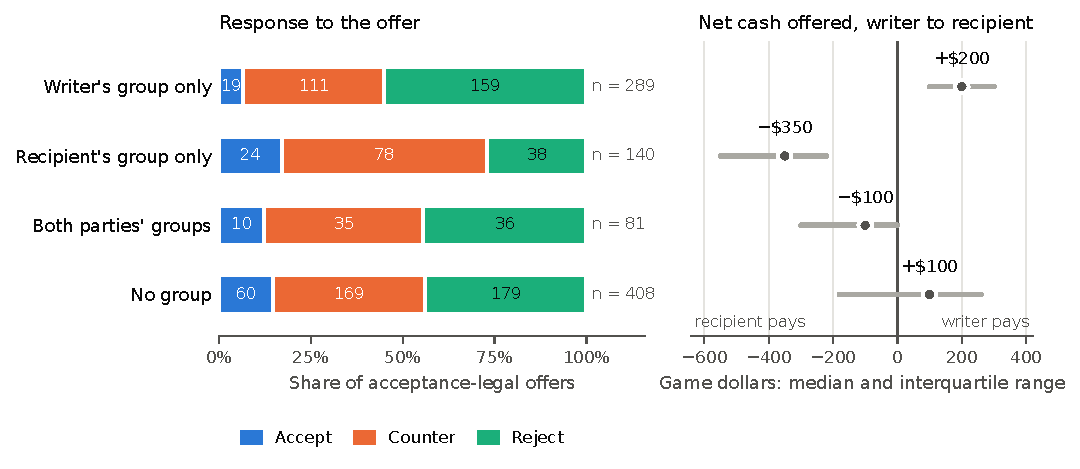
\includegraphics[width=\linewidth]{fig_bargaining.pdf}
\caption{All 918 acceptance-legal offers, by who would newly complete a color group if the offer were accepted. Left: the recipient's response, with counts. Right: net cash the writer offers the recipient (negative when the writer asks for cash). Rows are offers, not independent trials. The same thread, pair and game contribute many rows, and prices, holdings and responders differ across rows.}
\label{fig:bargaining}
\end{figure}

\subsection{Responses depend on who would complete}
\label{sec:cells}

Figure~\ref{fig:bargaining} (left) gives the response to every acceptance-legal offer. An offer that completes only the writer's group is accepted 19 times in 289 (7 percent) and rejected outright 159 times (55 percent). An offer that completes only the recipient's group is accepted 24 times in 140 (17 percent), countered 78 times (56 percent) and rejected 38 times (27 percent). Offers completing both sides' groups fall between the two, with 10 of 81 accepted and 36 rejected. Offers completing nothing are accepted 60 times in 408.

The figure does not measure the effect of a rival's completion on refusal. The rows differ in price, in what else changes hands, in who responds and in where the offer falls in a thread.

Position in the thread accounts for part of the contrast. Writer-only offers are mostly opening bids for the last deed a buyer needs (187 of 289 are first offers). Recipient-only offers are mostly a seller's counter that names a price (89 of 140 are later offers), and later offers are accepted more often everywhere. Within each position the difference keeps its direction and shrinks. Among first offers, writer-only offers are rejected 138 times in 187 and recipient-only offers 31 times in 51. Among later offers the rejections are 21 in 102 against 7 in 89, and the acceptances 16 in 102 against 22 in 89.

The direction of the rejection contrast is stable across the design. Writer-only offers are rejected at a higher rate than recipient-only offers in all five seed blocks and in 17 of the 19 games that contain both kinds. It holds for Sol, Gemini and Grok as recipients and not for Opus, which rejects almost nothing outright (3 of 52 against 6 of 42) and counters instead. The acceptance contrast is weaker and holds in four of five blocks and 13 of 19 games. Removing the eleven responses in which Grok's text and tool call disagree does not change the pattern (Appendix~\ref{app:bargaining}).

In this cohort, then, a proposal that would hand the proposer a monopoly is usually refused or repriced, and a proposal that would hand the recipient a monopoly at a price opens a negotiation more often than it closes one.

\subsection{Four ways of declining}

The systems accept at similar frequencies and differ in what they do otherwise (Table~\ref{tab:styles}). Each accepts between 26 and 30 offers, or 11 to 15 percent of those it receives. Sol and Opus mostly counter. Gemini and Grok mostly reject. Gemini rejects three offers in four outright and opens almost no threads of its own, yet it accepts about as many offers as any other system.

\begin{table}[t]
\centering\small
\begin{tabular}{lrrrrl}
\toprule
Recipient & Offers received & Accept & Counter & Reject & Response condition\\
\midrule
Sol & 235 & 30 & 140 & 65 & standard\\
Gemini & 242 & 26 & 36 & 180 & standard\\
Opus & 189 & 29 & 141 & 19 & action-only in 162\\
Grok & 254 & 28 & 77 & 149 & text and call disagree in 11\\
\midrule
All & 920 & 113 & 394 & 413 & \\
\bottomrule
\end{tabular}
\caption{Responses to all 920 offers, by recipient. Two offers lacked a legal acceptance (one to Gemini, rejected; one to Opus, countered). No response is an engine default. Seven of Grok's 28 acceptances come from tool calls whose text rejected or countered; without the eleven disagreeing responses its row reads 21, 76 and 146 of 243.}
\label{tab:styles}
\end{table}

Two rows carry conditions. Opus answered 162 of its 189 offers through the action-only path, with no private note. Three of the nineteen accepted writer-only offers are Grok tool calls that accepted while the text rejected, and all three completed a group for Opus. Low acceptance does not settle the worry, raised in studies of bilateral bargaining, that language models concede too readily~\cite{cosentino2026counterparty,shah2025rationalis}. A system could accept one offer in eight and still accept the wrong ones. The record shows only that agreement is not the default response of any of the four.

\subsection{Stated reasons for refusing one's own monopoly}
\label{sec:reasons}

Seventy-four acceptance-legal offers that would have completed the recipient's group were rejected outright. In 36 of them, accepting would also have completed a group for the writer, which is a fact of the ledger. What the recipients said is a matter of reading. All 74 have a public message and 66 have a private note. One language-model reading finds a stated consequence for the rival in 63 of the 74, such as the rival completing a set, gaining cash to build, or surviving. A second reading agrees on 61. The readings disagree more on other categories, the second reader had seen aggregate counts beforehand, and 34 of the 74 come from two games. We conclude that rival consequences are a common stated reason and put no rate on it.

Incident~\ref{inc:swap} shows one such refusal with its state.

\IncidentTitle{swap}{Refusing a monopoly because the other side could build first}

In game 15, turn 63, Sol (seat 4) has \$730, two of the three green deeds and two of the three yellow deeds. Grok (seat 2) has \$333, the third green and the third yellow. Gemini, by its own note, has three houses on each orange property. Sol proposes a swap that would complete yellow for itself and green for Grok:

\TranscriptQuote{fx-g15-offer}

Sol's private note on the same action states the asymmetry it is counting on:

\TranscriptQuote{fx-g15-offer-note}

Grok rejects, and says why in public:

\TranscriptQuote{fx-g15-refusal}

Its private note gives the arithmetic:

\TranscriptQuote{fx-g15-refusal-note}

The figures match the ledger. Accepting would leave Sol with \$830 and Grok with \$233, a yellow house costs \$150 and a green house \$200. Sol then drops the cash request and adds Kentucky Avenue, is rejected again, and finally offers to pay:

\TranscriptQuote{fx-g15-sweetener}

\TranscriptQuote{fx-g15-final-refusal}

\IncidentOutcome{No trade occurs. Grok is the first player eliminated, eighteen turns later, and its deeds, including the yellow and green blockers, pass to its creditor Gemini, who wins. Sol is eliminated last and never completes either group.}

\IncidentReading{Grok declines a complete color group three times, the last time with \$250 added, and each time for a stated reason about what Sol could do with the other half of the swap. Sol's private note shows it counting on the same asymmetry, and its third message addresses Grok's objection directly. Both sides reason about relative ability to build. The record does not show that refusing was the better choice. Grok went bankrupt first with the blockers still in hand, and a third player inherited them.}

\IncidentSource{G15 d168--175, turn 63. All quoted responses are standard first attempts. Cash and completion consequences are from the offer ledger. Elimination order and estate transfers are from the flow ledger. Appendix~\ref{app:incidents} gives a second refusal of this kind from a two-player endgame (G11).}

\subsection{Completing deeds are released by cash-poor holders}
\label{sec:cashpoor}

If holders refuse to sell the deed a rival needs, how do 63 groups get completed by trade? Mostly when the holder runs short of cash. Call the party that receives net cash in a settlement the seller. In the 48 settlements where the paying side completes a group, the seller's median cash before the offer was \$194, and in 21 it was under \$100. In the 57 settlements with a cash payment that complete nothing, the seller's median cash was \$571 and 9 sellers held under \$100. The \$100 line is arbitrary. At \$50 the completing sales number 14 of 20 cash-poor sales, and at \$200 they number 24 of 40. Across all 30 settlements with a seller under \$100, Opus is the seller in 16. Six of the 21 cash-poor sellers of a completing deed went on to win.

Being short of cash does not make a system easier to deal with (Table~\ref{tab:cashpoor}). Offers of cash to a recipient holding under \$100 are accepted about as often as other cash offers, 12 of 85 against 47 of 407. They are rejected outright much less often and countered much more. Requests for cash written by a player holding under \$100 are accepted as often as other requests (18 of 132 against 30 of 207) and rejected more often. Recipient style confounds these comparisons. We read them only as showing no surge of agreement when one side is nearly broke.

\begin{table}[t]
\centering\small
\begin{tabular}{lrrrr}
\toprule
Offer & Offers & Accept & Counter & Reject\\
\midrule
Cash offered to a recipient holding under \$100 & 85 & 12 & 55 & 18\\
Cash offered to any other recipient & 407 & 47 & 149 & 211\\
Cash requested by a writer holding under \$100 & 132 & 18 & 52 & 62\\
Cash requested by any other writer & 207 & 30 & 115 & 62\\
\bottomrule
\end{tabular}
\caption{Responses when the side that would receive net cash is short of it. Exploratory re-tabulation of the offer ledger for this draft, with the threshold fixed at \$100 before tabulating and other thresholds in Appendix~\ref{app:bargaining}. The remaining 87 acceptance-legal offers move no net cash.}
\label{tab:cashpoor}
\end{table}

Buyers' notes in these sales connect bargaining to the estate rule. In game 1, Opus has \$18 after mortgaging a railroad to pay rent and offers its mortgaged Boardwalk to Grok, who holds Park Place. Grok accepts at \$100 with this note:

\TranscriptQuote{fx-g1-boardwalk-note}

The note gives Grok's reason for paying above its own ceiling: Opus's bankruptcy would hand the deed to a third player. Opus is eliminated four turns later and its estate goes to that player, Gemini. Grok's dark-blue group stays mortgaged and unbuilt in its first management window. It is one of the encumbered completions counted in Section~\ref{sec:development}.

\subsection{What a settlement does and does not show}

Two short incidents mark the limits of reading a settlement, and Appendix~\ref{app:incidents} holds further cases.

\IncidentTitle{abort}{A false premise corrected, and the deal accepted anyway}

In game 19, Grok's applied tool call proposes Virginia Avenue plus \$150 for Sol's States Avenue, with this message:

\TranscriptQuote{g19_d135_false_public}

Both deeds are pink, so the claim about orange is false. The private note attached to the same response says so and says not to send the trade:

\TranscriptQuote{g19-abort}

The assistant text of that response names \End{} as the action. Sol answers:

\TranscriptQuote{g19_d136_correction_accept}

\IncidentOutcome{The trade executes. Grok pays \$150 and the two pink deeds change hands.}

\IncidentReading{The recipient states that the premise is false and accepts on the terms, so acceptance is no evidence that the claim was believed. On the proposer's side the text, the note and the tool call disagree, so the false message cannot be read as a plan to mislead. This is one of the 60 Grok proposals sent by a tool call while the text ended the turn.}

\IncidentSource{G19 d135--136, turn 67, standard first attempts. Sol's prompt contains the false claim. Its applied note also treats States Avenue as pink.}

\IncidentTitle{final}{A public final price below the private limit}

In game 7, Grok wants North Carolina Avenue from Sol. Sol has just asked \$625. Grok presents its bid as the last one:

\TranscriptQuote{g7_d42_public}

The private note on the same response leaves room:

\TranscriptQuote{g7_d42_private}

Sol accepts:

\TranscriptQuote{g7_d43_public}

\IncidentOutcome{Sol transfers the deed for \$600. Its note says it prefers to reinvest in cheaper sets than hold out for another \$25. Grok's note shows it would have paid the \$625 that Sol had asked.}

\IncidentReading{This is a bluff about a reservation price, stated in one channel and contradicted in the other, in a task that permits bluffing. The \$25 that Sol gave up is within the room Grok's note left. Whether the word ``final'' secured it is unknown, because the same offer without it was never made.}

\IncidentSource{G7 d41--43, turn 25, standard first attempts. Sol's \$625 counter at d41 was checked in the decision log for this draft. Sol's prompt contains the \$600 message.}
